\subsection{Messschaltung}

Um die Ausgangskennlinie regeln zu können, müssen die Ausgangsgrössen Spannung (in der Software als $istU$ bezeichnet) und Strom (in der Software als $istI$ bezeichnet) bekannt sein. Die Eingänge des Mikrocontrollers können aber nur Spannungen im Bereich zwischen 0V und 5V mit einer Genauigkeit von 10bit messen. Folglich wird eine Schaltung benötigt, welchen den Spannungsbereich 0V bis 24V und den Strombereich 0A bis 3.5A jeweils auf den Spannungsbereich zwischen 0V und 5V anpassen. Im folgenden Abschnitt wird genauer auf diese Schaltung eingegangen, welche in Abbildung \ref{fig:Messschaltung} dargestellt ist.
\begin{figure}[h]
	\centering
		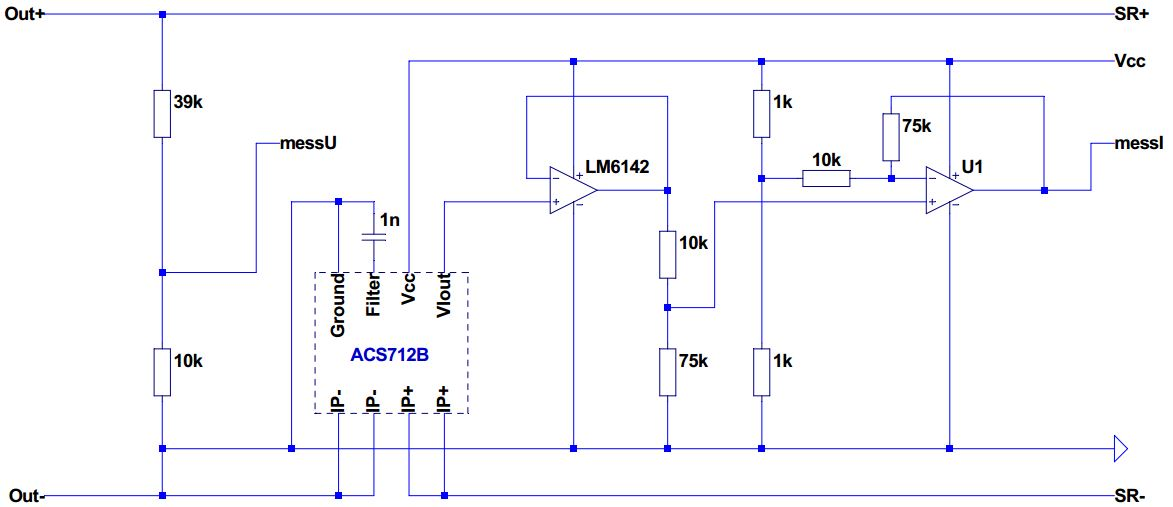
\includegraphics[width=1.00\textwidth]{Messschaltung.JPG}
	\caption{Die komplette Messschaltung.}
	\label{fig:Messschaltung}
\end{figure}


\subsubsection{Spannungsmessung}
\begin{figure}[h]
	\centering
		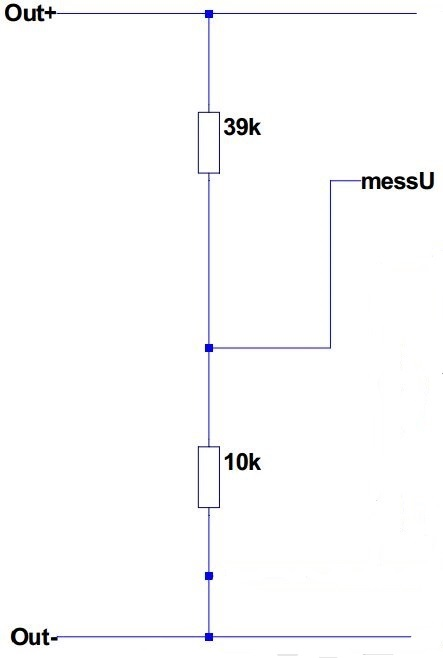
\includegraphics[width=0.30\textwidth]{Messschaltung_U.JPG}
	\caption{Die Messschaltung zur Spannungsmessung.}
	\label{fig:Messschaltung_U}
\end{figure}

Um die Spannung am Ausgang messen zu können, wird ein Spannungsteiler benötigt. Im einfachsten Fall kann ein Spannungsteiler aus zwei Widerständen bestehen, Abbildung \ref{fig:Messschaltung_U} zeigt diesen Spannungsteiler. Die Spannung $messU$ berechnet sich nach folgender Formel:
\begin{equation}
	messU=\frac{\Delta U\cdot R_2}{R_1+R_2}=\frac{U_{Out}\cdot10k\Omega}{39k\Omega +10k\Omega}=\frac{U_{Out}}{4.9}
\label{eq:messU}
\end{equation}
 Die beiden Widerstände sollten dabei folgende Bedingungen erfüllen:
\begin{itemize}
	\item Da innerhalb der Messschaltung selbst eine Spannung abfallen kann ist es wichtig, die Spannungsmessung möglichst nahe am Ausgang vorzunehmen.
	\item Um bei 24V Ausgangsspannung am Ausgang des Spannungsteiler 5V zu erhalten, sollte das Ver\-hält\-nis der Widerstände ungefähr $\frac{R_1}{R_2}=3.8$ betragen.
	\item Die Widerstände sollten nicht zu klein dimensioniert werden, um die Schaltung nicht zu belasten.
	\item Die Widerstände sollten nicht zu gross dimensioniert werden, sodass der Eingang des Mikrocontrollers die Messung nicht verfälscht.
\end{itemize}
Aus diesem Grund wurde $R_1=39k\Omega$ und $R_2=10k\Omega$ gewählt. Damit die Schaltung reproduzierbar gestaltet werden kann, wurden Metallschichtwiderstände mit einer Genauigkeit von $\pm 1\%$ verwendet. Die Genauigkeit der Schaltung wurde ausserdem mit einer Messreihe \ref{subsec_messu} auf Seite \pageref{subsec_messu} verifiziert.

\subsubsection{Strommessung}
\begin{figure}[h]
	\centering
		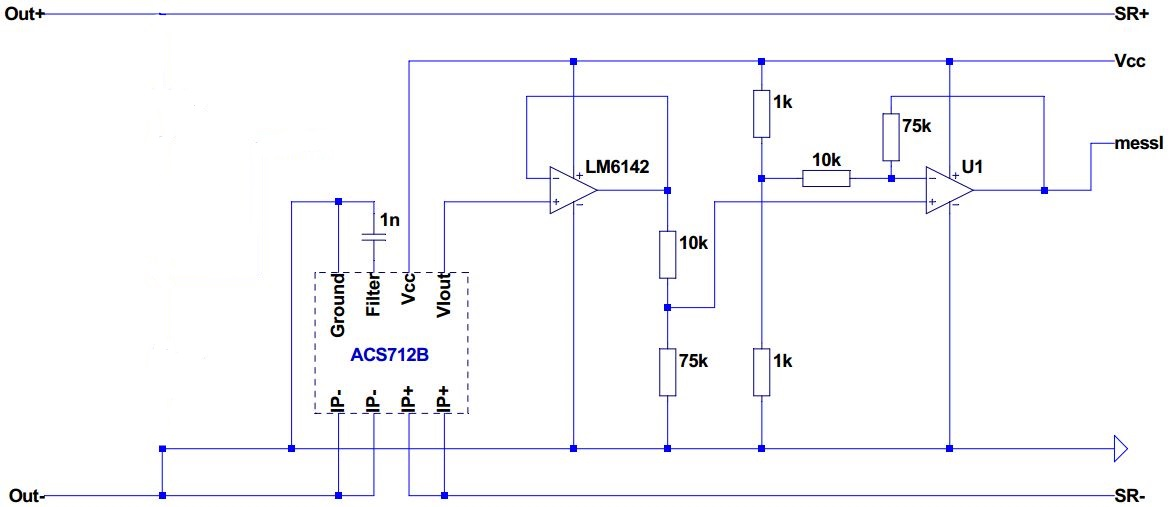
\includegraphics[width=1.00\textwidth]{Messschaltung_I.JPG}
	\caption{Die Messschaltung zur Strommessung.}
	\label{fig:Messschaltung_I}
\end{figure}
Die Messung des Stromes wird oftmals mit einem Shuntwiderstand bestimmt, über dem der Spannungsabfall gemessen wird. Da dies jedoch zwangsläufig mit Verlusten verbunden ist und ausserdem die Ausgangsspannung abhängig vom Strom verfälscht, wurde ein Hallsensor gewählt, der diese Nachteile nicht besitzt. Hallsensoren liefern eine Ausgangsspannung, die proportional zum Produkt aus magnetischer Feldstärke und Strom ist. Da die magnetische Feldstärke konstant ist, ist die Ausgangsspannung proportional zum Strom.

Der ACS712B von Allegro MicroSystems \cite{db_acs712} besitzt eine Sensitivität von 185mV/A sowie einen Spannungsoffset von Vcc/2. Diese Spannung wird, da der Ausgangswiderstand des ACS712B mit mindestens 4.7k$\Omega$ eher hoch ist, zuerst in einer Impedanzwandlerschaltung mit einem Operationsverstärker niederohmig gemacht. Bei einem Strombereich von 0A bis 3.5A wird dabei lediglich ein Spannungsbereich von 2.5V bis 1.85V ausgenutzt. Aus diesem Grund wird die Ausgangsspannung des ACS712B zuerst mit einer Subtraktionsschaltung vom Offset bereinigt, wodurch ein Spannungsbereich von -0.65V bis 0.0V entsteht. Anschliessend wird diese Spannung um den Faktor -7.5 verstärkt, sodass der Spannungsbereich des Einganges des Mikrocontrollers voll ausgenutzt werden kann. Das Bereinigen vom Offset und die Spannungsverstärkung kann mit einem einzigen Operationsverstärker umgesetzt werden. Dies bringt ausserdem den Vorteil, das keine negative Versorgungsspannung benötigt wird. Die Widerstandswerte sollten dabei nicht zu klein sein, damit die Ausgänge nicht zu sehr von den Widerständen belastet werden. Die Widerstandswerte sollten aber auch nicht zu gross sein, sodass die Schaltung genügend Strom für die Eingänge der Operationsverstärker beziehungsweise des Mikrocontrollers liefern kann.  Die theoretischen Grundlagen zu den Operationsverstärkerschaltungen können in \cite{operationsverstaerker} nachgelesen werden. Die Spannung $messI$ kann mit folgender Formel berechnet werden:
\begin{equation}
	messI=\left(\frac{Vcc}{2}-185mV\cdot I_{Out}-\frac{Vcc\cdot 1k\Omega}{1k\Omega +1k\Omega}\right)\cdot -\frac{75k\Omega}{10k\Omega}=1.3875\cdot I_{Out}
\label{eq:messI}
\end{equation}

Für diese Anpassung des Messresultates werden zwei Operationsverstärker benötigt. Die Auswahl des Operationsverstärkers erfolge nach folgenden Kriterien:
\begin{itemize}
	\item Nach Möglichkeit sollten beide Operationsverstärker in einem Gehäuse verbaut sein.
	\item Der Operationsverstärker sollte mit einer einseitigen Speisung von 5V betrieben werden können.
	\item Die Ausgangsspannung des Operationsverstärker sollte den kompletten Bereich von 0V bis 5V ausnützen können, aus diesem Grund sollte ein Rail-To-Rail Design verwendet werden.
\end{itemize}
Aus diesen Gründen wurde das Modell LM6142BIN von National Semiconductor gewählt. Die Genauigkeit der Schaltung wurde ausserdem mit einer Messreihe \ref{subsec_messi} auf Seite \pageref{subsec_messi} verifiziert.